\documentclass[11pt,a4paper]{article}

\usepackage[T1]{fontenc}
\usepackage[utf8]{inputenc}
\usepackage[spanish,es-noshorthands]{babel}
\usepackage{lmodern}
\usepackage{amsmath,amssymb}
\usepackage[margin=2.4cm]{geometry}
\usepackage{booktabs}
\usepackage{graphicx}
\usepackage{microtype}
\usepackage{enumitem}
\usepackage[colorlinks=true,linkcolor=black,citecolor=black,urlcolor=blue]{hyperref}

\graphicspath{{figuras_variantes/}}

\newcommand{\dd}{\,\mathrm{d}}
\newcommand{\p}{\partial}
\newcommand{\vin}{v_{\mathrm{in}}}
\newcommand{\MPa}{\ensuremath{\,\mathrm{MPa}}}
\newcommand{\ms}{\ensuremath{\,\mathrm{m/s}}}
\newcommand{\Pam}{\ensuremath{\,\mathrm{Pa/m}}}

\title{\vspace{-1.2cm}\textbf{Variantes del cierre después de la fragmentación}\\[0.3em]
\large Conducto 2D, Calbuco 2015}
\author{Ignacio Gómez Gómez}
\date{\today}

\begin{document}
\maketitle
\vspace{-0.8cm}

\begin{abstract}\noindent
Bitácora de las variantes ya corridas para el tramo fragmentado del
conducto bidimensional. Cada sección fija las ecuaciones, la corrida
y la figura. El caso es el de Calbuco 2015: cilindro de radio
$R=16\,\mathrm{m}$, profundidad $H=-7000\,\mathrm{m}$,
$\phi_{\mathrm{crit}}=0{,}7$, $P_{\mathrm{atm}}=10^{5}\,\mathrm{Pa}$,
$T=1173{,}15\,\mathrm{K}$, cristalinidad de entrada $\xi_0=0{,}25$,
$\tau_{\mathrm{car}}=2\,\mathrm{h}$ y arrastre $C=300\,\mathrm{m}^{-1}$.
\end{abstract}

\tableofcontents
\vspace{0.5em}

\section{Tramo común, antes de fragmentar}

En todas las variantes el conducto por debajo de la fragmentación es el
mismo. La velocidad del fundido $u_m(r)$ sale del algoritmo de Thomas.
El gas va trabado, $u_g=u_m$. La fracción de gas es la de Henry con la
cristalinidad local,
\[
\phi=\phi_{\mathrm{Henry}}(P,\xi),
\]
y $\xi(r)$ y el número de burbujas $N(r)$ se integran con su cinética.
Con $\tau_{\mathrm{car}}=2\,\mathrm{h}$ el ascenso dura del orden de un
minuto, así que $\xi$, $N$ y $\phi$ casi no cambian con el radio: la
presión es una sola en la sección y la cristalización no alcanza a
diferenciar los radios.

A partir de $z_f$ las variantes se separan. En todas se congela el
flujo másico que trae Thomas,
\[
q(r)=\rho_m(1-\phi_f)\,u_{m,f}+\rho_g(z_f)\,\phi_f\,u_{g,f},
\]
y el reparto entre líquido y gas se evalúa sin cristales en el factor
de masa del gas, porque los cristales quedan en el líquido:
\[
n(P)=\frac{1}{1+\dfrac{\rho_g(P)}{\rho_m}\left(\dfrac{1}{c_g(P)}-1\right)}.
\]
El salto de $u_g$ justo al fragmentar, del orden de
$1/(1-\xi_0)=4/3$, es el paso de la fórmula de masa con $\xi$ a esta
fórmula.

\section{Promedio de sección}
\label{sec:media}

Una sola presión $P(z)$ y una sola fracción $\bar\phi(z)$. Con el
promedio $\bar q$ las velocidades de la sección son
\[
\bar u_m=\frac{(1-n)\,\bar q}{\rho_m(1-\bar\phi)},\qquad
\bar u_g=\frac{n\,\bar q}{\rho_g\,\bar\phi},
\]
y el sistema es
\begin{align}
\rho_m\bar u_m\frac{\dd\bar u_m}{\dd z}+\frac{\dd P}{\dd z}+\rho_m g
  -\frac{F_{mg}}{1-\bar\phi}&=0, \label{eq:mom-m}\\[4pt]
\rho_g\bar u_g\frac{\dd\bar u_g}{\dd z}+\frac{\dd P}{\dd z}+\rho_g g
  +\frac{F_{mg}}{\bar\phi}&=0, \label{eq:mom-g}
\end{align}
con
$F_{mg}=C\,\phi(1-\phi)(u_g-u_m)|u_g-u_m|$.
De~\eqref{eq:mom-m}--\eqref{eq:mom-g} salen $\dd P/\dd z$ y
$\dd\bar\phi/\dd z$. Las velocidades de cada radio se reconstruyen con
el mismo $n$ y el $q(r)$ congelado, así que el perfil de Thomas se
conserva por encima de $z_f$.

El tiro de esta variante está en la sección~\ref{sec:tiro}: con
$\vin=16{,}133\ms$ la media llega sónica a la boca.

\section{Cada radio pide otra pendiente}
\label{sec:pendientes}

Si el sistema $2\times 2$ se escribe en cada radio, con su $q(r)$ y sin
promediar, $\dd P/\dd z$ deja de ser único. Sustituyendo
\[
u_m=\frac{(1-n)\,q(r)}{\rho_m(1-\phi)},\qquad
u_g=\frac{n\,q(r)}{\rho_g\,\phi}
\]
en los dos momentos, cada radio tiene su propio par
$(P(r,z),\,\phi(r,z))$.

\paragraph{Corrida.}
$\vin=17{,}021\ms$. Fragmentación en $z_f=-906{,}2\,\mathrm{m}$,
$P_f=12{,}00\MPa$, $\phi_f=0{,}702$.

\begin{table}[ht]
\centering
\caption{Flujo másico congelado y pendiente de presión que pide cada
radio en $z_f$. El promedio de la sección pide
$\dd P/\dd z=-5{,}8\times 10^{5}\Pam$.}
\label{tab:dpdz}
\begin{tabular}{@{}lrr@{}}
\toprule
radio & $q$ [$\mathrm{kg\,m^{-2}s^{-1}}$] & $\dd P/\dd z$ [\Pam] \\
\midrule
eje            & $9{,}41\times 10^{4}$ & $-3{,}77\times 10^{6}$ \\
medio          & $5{,}76\times 10^{4}$ & $-1{,}38\times 10^{6}$ \\
cerca de la pared & $6{,}91\times 10^{3}$ & $-2{,}30\times 10^{4}$ \\
\bottomrule
\end{tabular}
\end{table}

El eje lleva unas catorce veces más masa que la pared y pide una
descompresión dos órdenes más fuerte. Una sola $P(z)$ no cumple el
momento en todos los radios a la vez.

\section{Integración local del eje}
\label{sec:eje}

Se integró el $2\times 2$ del eje con $q(0)$ congelado y $n(P)$ sin
$\xi$. La marcha es la de Euler.

\paragraph{Resultado.}
Con la fragmentación en $z_f=-906\,\mathrm{m}$ ($P_f=12\MPa$,
$u_{g,f}=67\ms$, $u_{m,f}=16\ms$) el eje se detiene en
$z=-905\,\mathrm{m}$. Ahí $P=8{,}59\MPa$, $u_g=757\ms$,
$u_m=65\ms$ y $\phi=0{,}841$. Un metro de ascenso lleva el gas de
$67\ms$ a la velocidad del sonido.

\begin{figure}[ht]
\centering
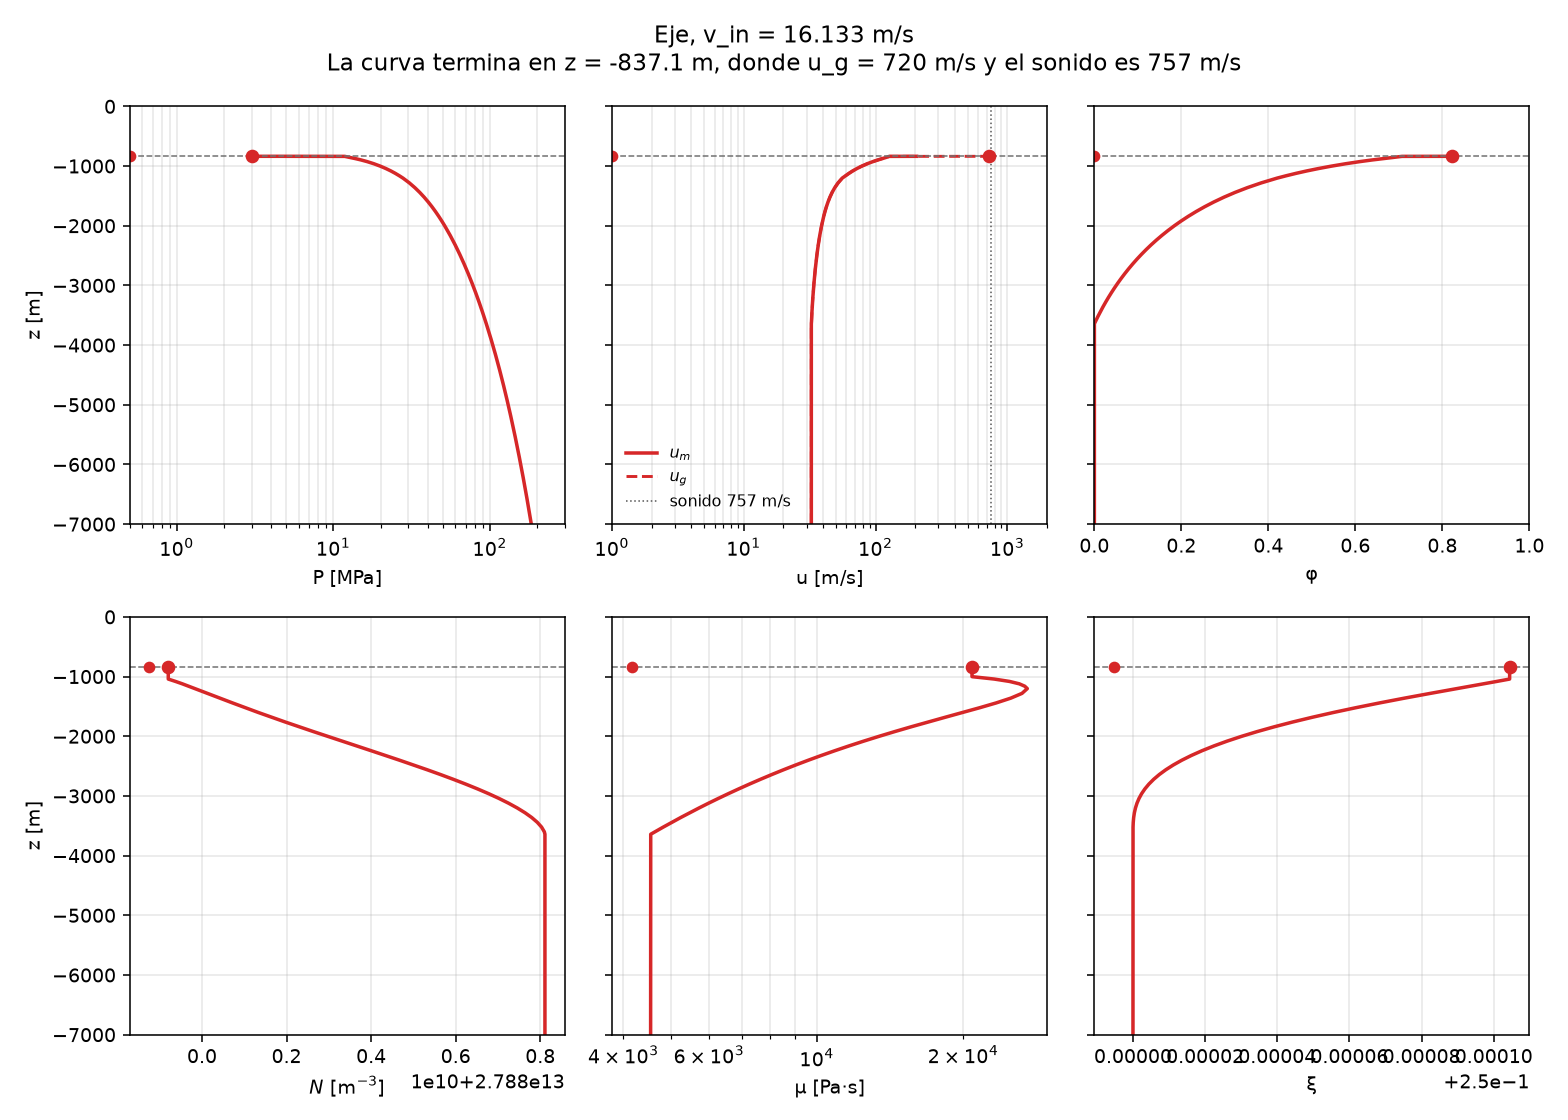
\includegraphics[width=\textwidth]{perfiles-eje.png}
\caption{Eje, integración local. La columna se corta en
$z=-905\,\mathrm{m}$, un metro sobre la fragmentación
($z_f=-906\,\mathrm{m}$), cuando $u_g$ llega a $757\ms$.}
\label{fig:eje}
\end{figure}

\section{Laplaciano viscoso del gas}
\label{sec:lap}

Al momento del gas se le sumó
\[
L_r=\frac{1}{r}\frac{\p}{\p r}\!\left(
  r\,\mu_g\,\phi\,\frac{\p u_g}{\p r}\right),
\qquad \mu_g=10^{-5}\,\mathrm{Pa\cdot s},
\]
de modo que el segundo miembro de~\eqref{eq:mom-g}, escrito en el
radio, gana el término $-L_r/\phi$.

\paragraph{Resultado.}
En la fragmentación de la corrida anterior
($z_f=-906{,}2\,\mathrm{m}$, $\vin=17{,}021\ms$) se mide
$|L_r|_{\max}=4{,}6\times 10^{-3}\Pam$, dentro de la banda
$10^{-5}$--$10^{-3}\Pam$. Al lado de
$\dd P/\dd z\sim 10^{6}\Pam$ el término no mueve los perfiles: el eje
sigue cortándose al hacerse sónico y la pared llega a $z=0$ subsónica.
La figura~\ref{fig:lap} trae las tres columnas (eje, radio medio y
pared) con $L_r$ incluido.

\begin{figure}[ht]
\centering
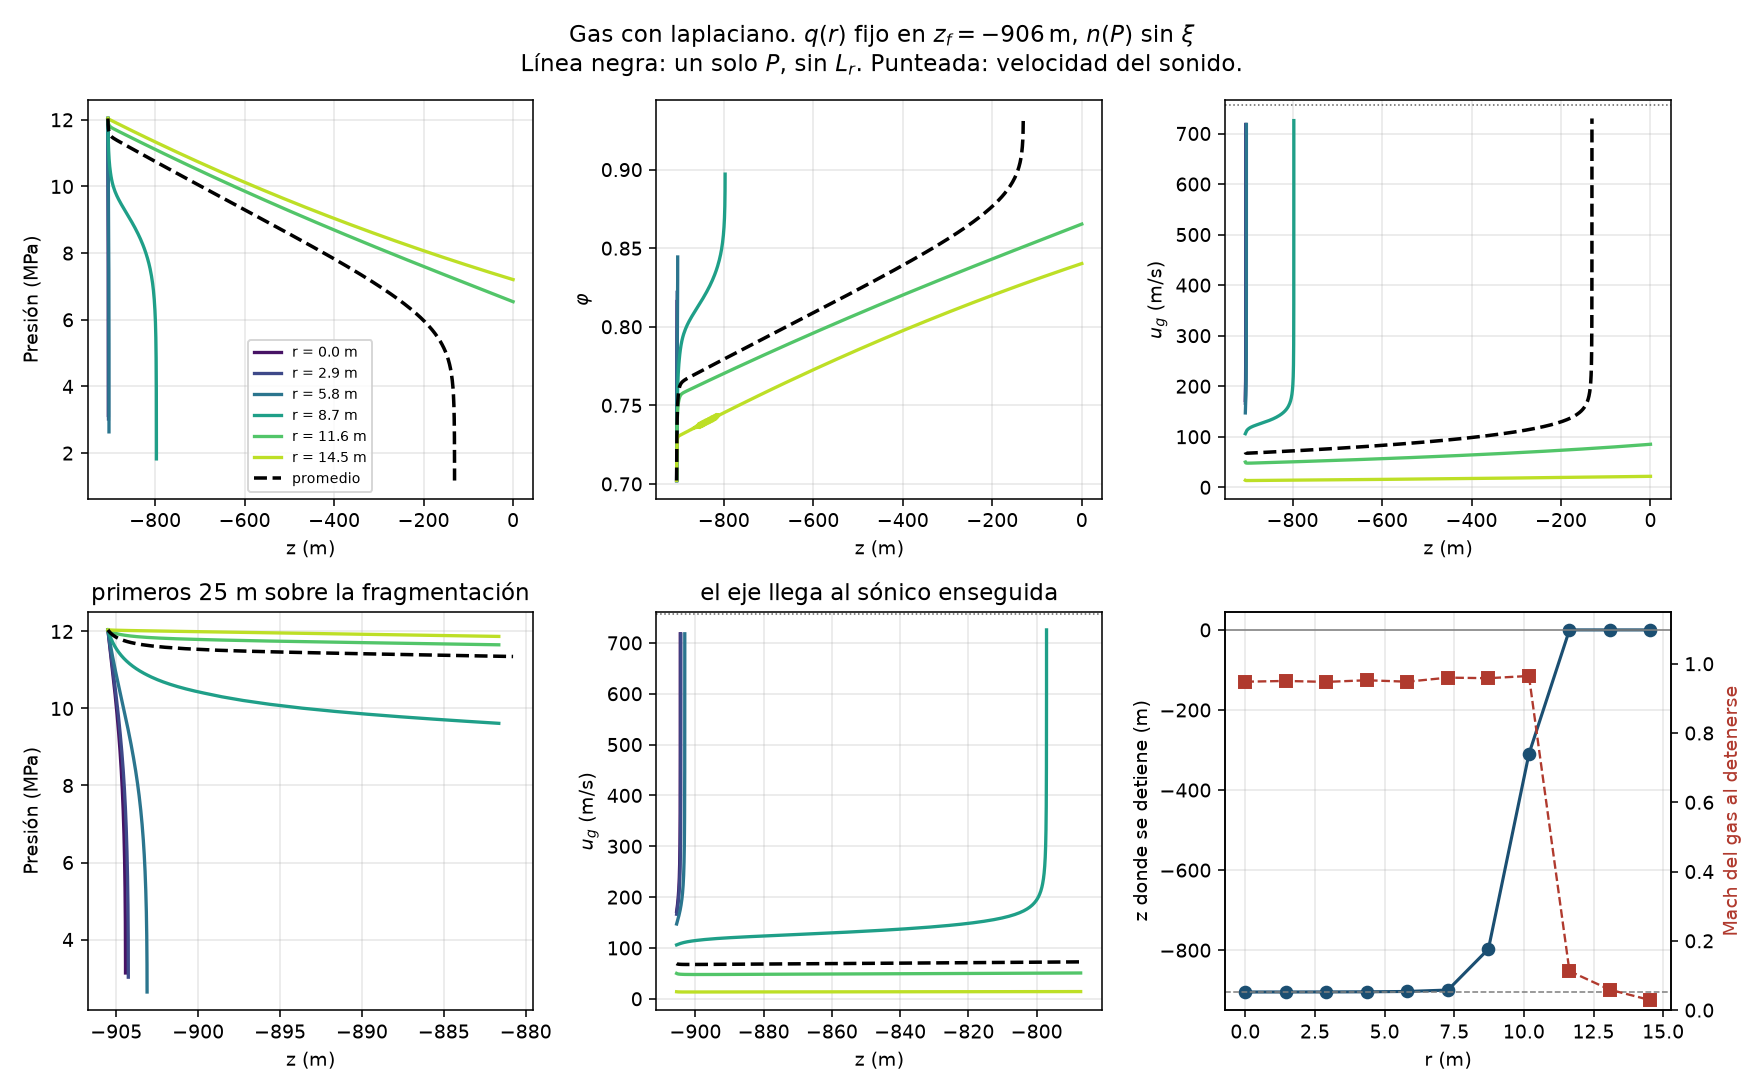
\includegraphics[width=\textwidth]{edp-local-con-laplaciano.png}
\caption{Sistema local con el laplaciano del gas,
$\mu_g=10^{-5}\,\mathrm{Pa\cdot s}$.
$|L_r|_{\max}=4{,}6\times 10^{-3}\Pam$ en $z_f=-906{,}2\,\mathrm{m}$.
Arriba, de izquierda a derecha: $\phi$, $P$, $u_m$ y $u_g$ frente a
$z-z_f$. Abajo: $q(r)$ y $\dd P/\dd z$ en la fragmentación, y $|L_r|$
en ese mismo nivel.}
\label{fig:lap}
\end{figure}

\section{Tiro de la media}
\label{sec:tiro}

El tiro busca el $\vin$ que deja $\bar u_g$ sónica en la boca, con el
cierre de la sección~\ref{sec:media}.

\paragraph{Resultado.}
Converge en $\vin=16{,}133\ms$. La fragmentación queda en
$z_f=-838\,\mathrm{m}$, con $u_{g,f}=51{,}1\ms$. La media llega a
$z=-0{,}44\,\mathrm{m}$ con $P=1{,}11\MPa$ y $\bar u_g=730\ms$.

\begin{figure}[ht]
\centering
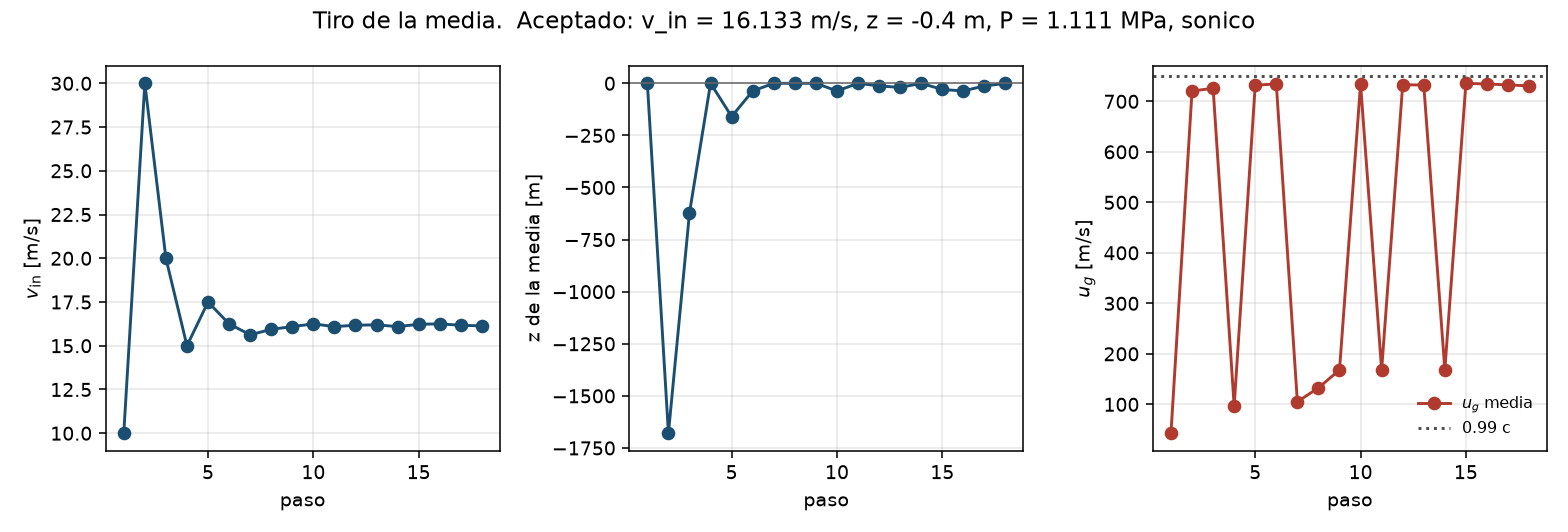
\includegraphics[width=0.72\textwidth]{tiro-vin.png}
\caption{Tiro sobre la velocidad media del gas. $\vin=16{,}133\ms$,
boca en $z=-0{,}44\,\mathrm{m}$ con $P=1{,}11\MPa$ y
$\bar u_g=730\ms$.}
\label{fig:tiro}
\end{figure}

Ese $\vin$ fija la sección. El eje, integrado con su propio $2\times 2$
y el mismo $q(0)$, se ahoga igual, un metro sobre $z_f$. La
figura~\ref{fig:eje-borde} muestra la columna completa del eje y del
radio $r=13{,}1\,\mathrm{m}$.

\paragraph{Resultado en el eje y cerca de la pared.}
Fragmentación común en $z_f=-838\,\mathrm{m}$, $P_f=10\MPa$,
$u_{g,f}=51\ms$. El eje se detiene en $z=-837\,\mathrm{m}$ con
$P=7{,}15\MPa$, $u_g=757\ms$, $u_m=49\ms$ y $\phi=0{,}866$.
El radio $r=13{,}1\,\mathrm{m}$ llega a $z=0$ con $P=6{,}95\MPa$,
$u_g=80\ms$, $u_m=5{,}2\ms$ y $\phi=0{,}871$.

\begin{figure}[ht]
\centering
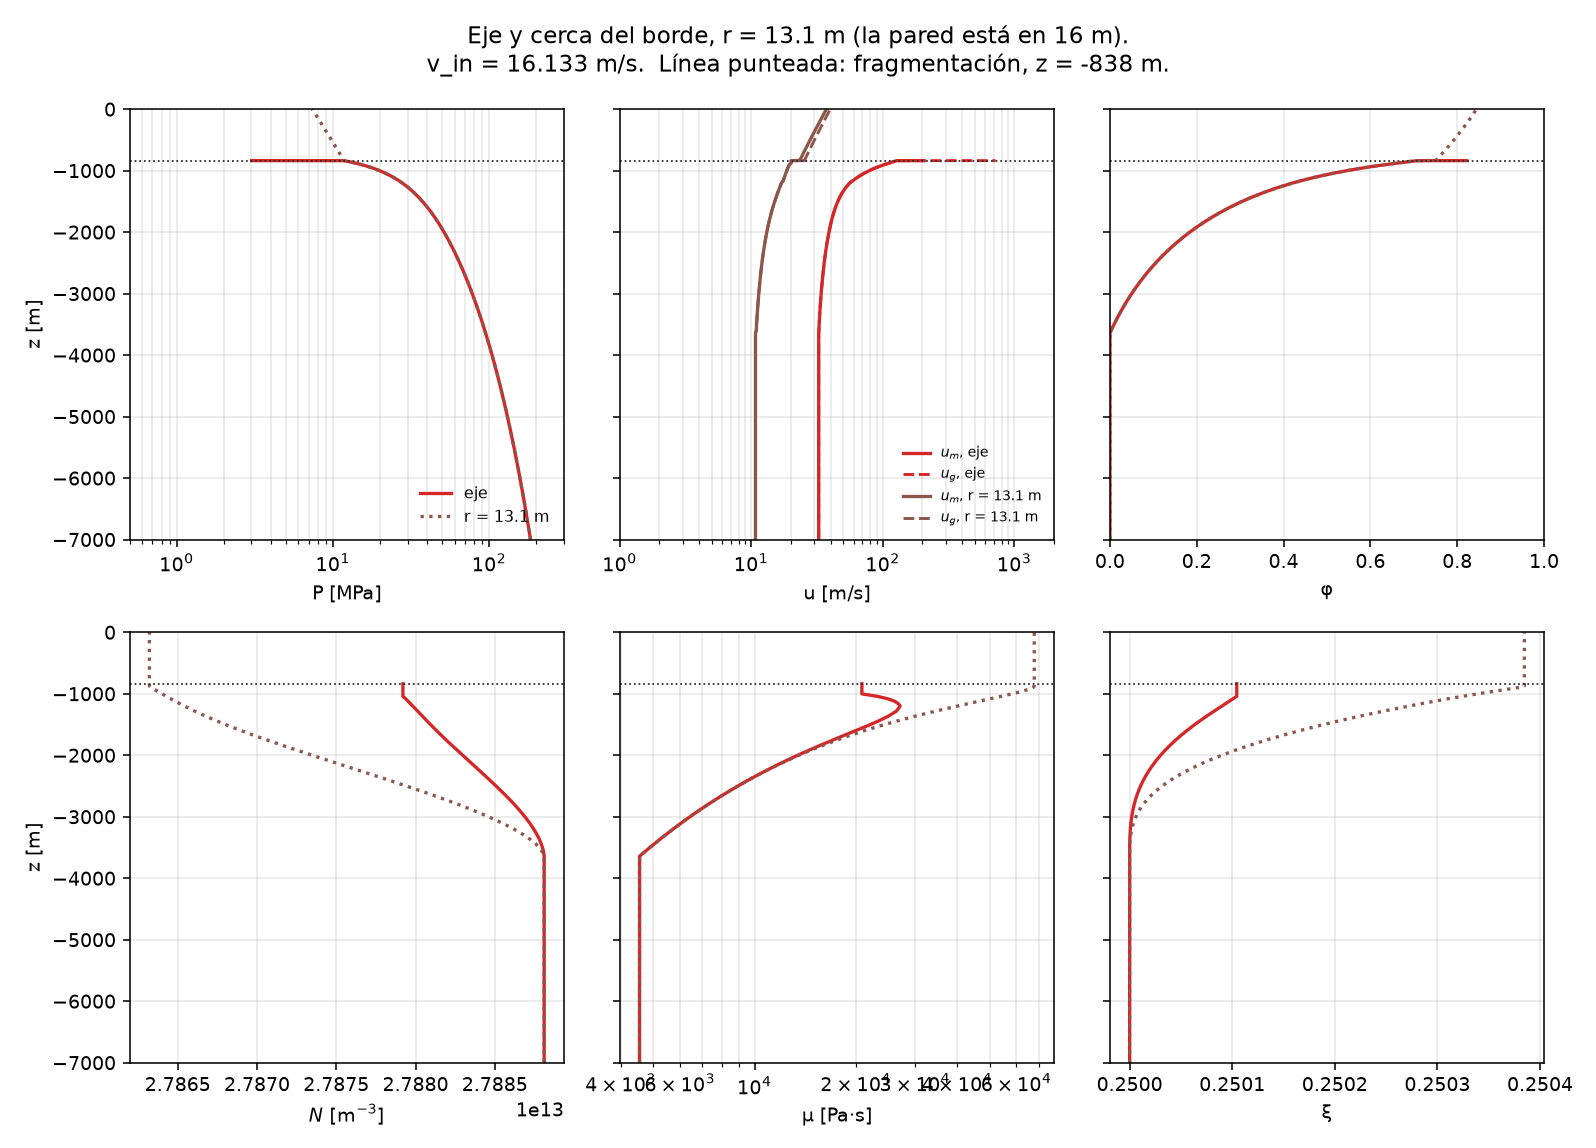
\includegraphics[width=\textwidth]{perfiles-eje-borde.png}
\caption{Columna con $\vin=16{,}133\ms$. Azul: eje, cortado en
$z=-837\,\mathrm{m}$ al llegar $u_g$ a $757\ms$. Naranjo:
$r=13{,}1\,\mathrm{m}$, que alcanza la boca a $80\ms$ y
$6{,}95\MPa$.}
\label{fig:eje-borde}
\end{figure}

\section{Diferencias hacia atrás}
\label{sec:fd}

En cada paso de altura $h$ se resuelve con \texttt{least\_squares} el
sistema implícito en $(u_m,u_g,P,\phi)$ del nivel nuevo:
\begin{align*}
\rho_m\frac{u_{m,j}^{2}-u_{m,j-1}^{2}}{2h}
  +\frac{P_j-P_{j-1}}{h}+\rho_m g
  -\frac{F_{mg,j}}{1-\phi_j}&=0,\\[6pt]
\rho_g\frac{u_{g,j}^{2}-u_{g,j-1}^{2}}{2h}
  +\frac{P_j-P_{j-1}}{h}+\rho_g g
  +\frac{F_{mg,j}}{\phi_j}
  -\frac{L_{r,j}}{\phi_j}&=0.
\end{align*}
Cerca de la singularidad sónica el paso baja hasta
$10^{-5}\,\mathrm{m}$.

\paragraph{Resultado.}
El eje, con el $\vin$ del tiro, se detiene en $z=-837{,}3\,\mathrm{m}$.
Ahí $P=7{,}23\MPa$, $u_g=718\ms$, $u_m=47\ms$ y $\phi=0{,}864$.
Euler, en la figura~\ref{fig:eje-borde}, corta el mismo eje en
$z=-837\,\mathrm{m}$ con $u_g=757\ms$ y $P=7{,}15\MPa$. Los dos
esquemas paran en el mismo metro: el corte es la condición sónica, no
el método.

\begin{figure}[ht]
\centering
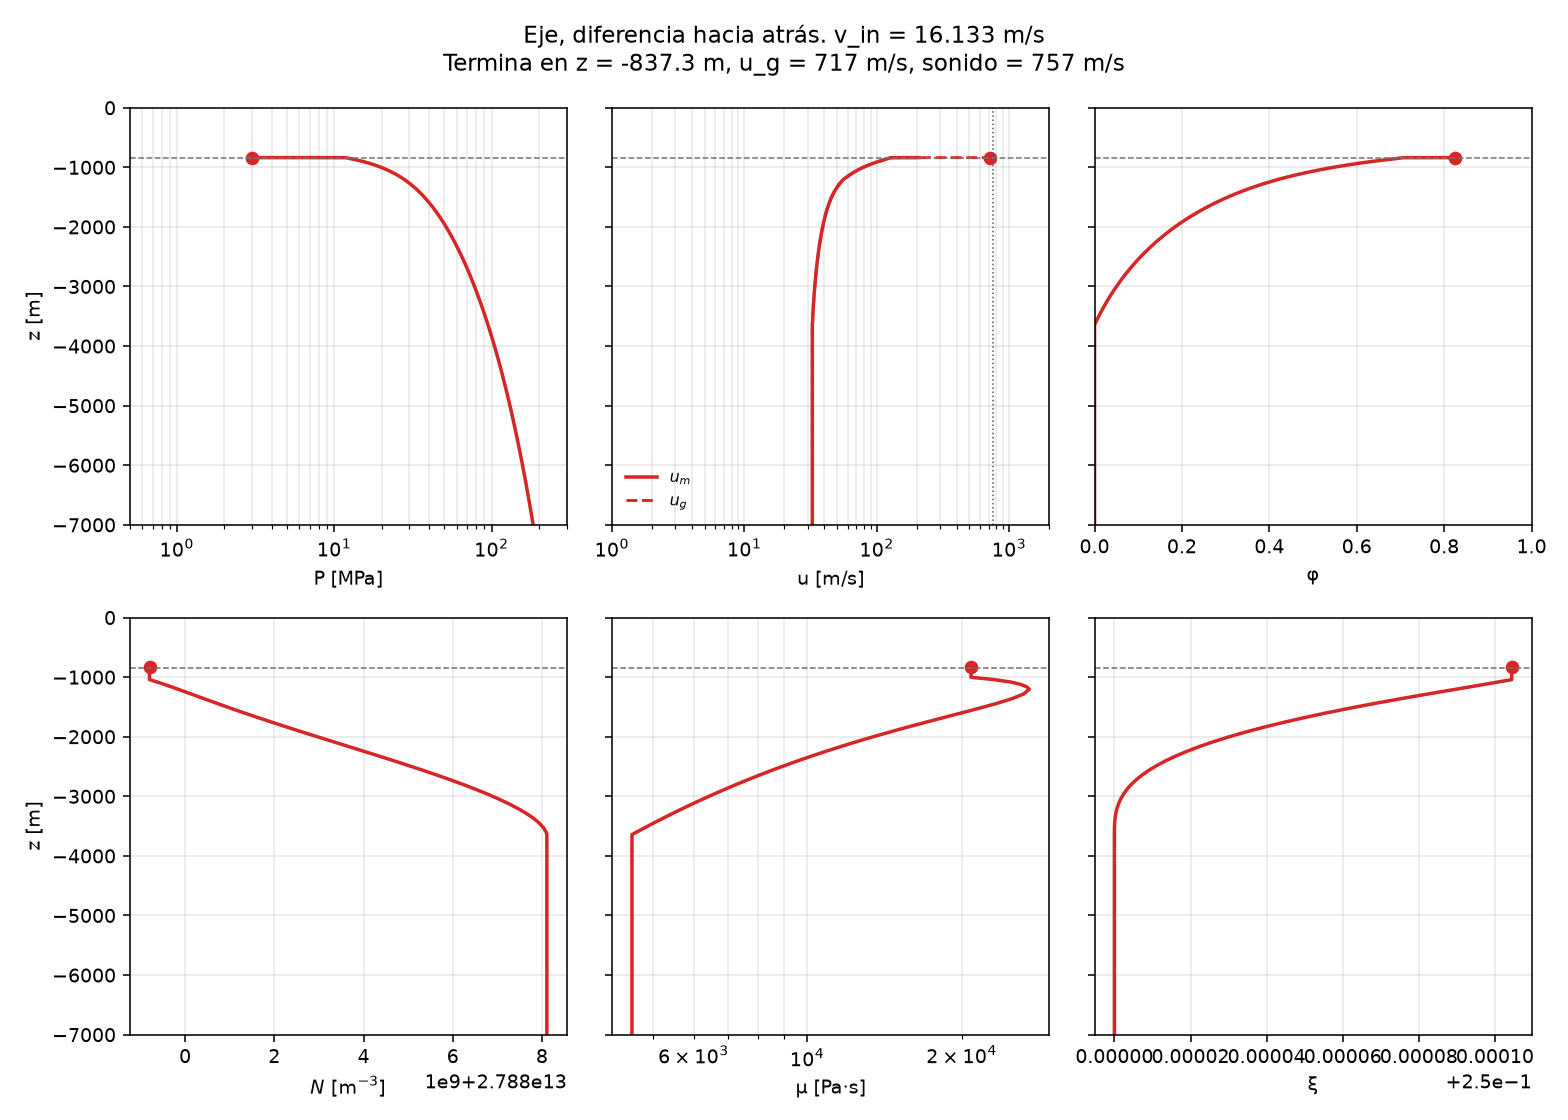
\includegraphics[width=\textwidth]{perfiles-eje-fd.png}
\caption{Eje con diferencias hacia atrás. $z_f=-838\,\mathrm{m}$,
$P_f=10\MPa$, $u_{g,f}=51\ms$. El último nivel aceptado es
$z=-837{,}3\,\mathrm{m}$, con $u_g=718\ms$ y $P=7{,}23\MPa$.}
\label{fig:fd}
\end{figure}

\section{Radios que siguen después del eje}
\label{sec:radios}

Cuando un nodo llega a $u_g$ sónica sale del vector activo y el resto
sigue subiendo, con el mismo esquema de la sección~\ref{sec:fd}.

\paragraph{Resultado.}
Los cinco radios interiores se congelan sónicos entre
$z=-837{,}3\,\mathrm{m}$ y $z=-153\,\mathrm{m}$. Los dos exteriores
llegan a la boca subsónicos, con presiones de $6{,}9$ y $7{,}4\MPa$.
Cada radio termina con su propia presión.

\begin{table}[ht]
\centering
\caption{Estado en el que se detiene cada radio al congelar los nodos
sónicos. Diferencias hacia atrás, $\vin=16{,}133\ms$.}
\label{tab:radios}
\begin{tabular}{@{}rrrrp{4.6cm}@{}}
\toprule
$r$ [m] & $z$ final [m] & $P$ [\MPa] & $u_g$ [\ms] & estado \\
\midrule
$0{,}0$  & $-837{,}3$ & $7{,}23$ & $718$ & sónico, congelado \\
$2{,}9$  & $-837{,}2$ & $7{,}28$ & $699$ & sónico, congelado \\
$5{,}8$  & $-836{,}0$ & $8{,}05$ & $557$ & sónico, congelado \\
$8{,}7$  & $-671{,}6$ & $9{,}48$ & $160$ & sónico, congelado \\
$10{,}2$ & $-153{,}1$ & $8{,}86$ & $92$  & sónico, congelado \\
$11{,}6$ & $0{,}0$    & $6{,}86$ & $74$  & subsónico, en la boca \\
$13{,}1$ & $0{,}0$    & $7{,}39$ & $40$  & subsónico, en la boca \\
\bottomrule
\end{tabular}
\end{table}

\begin{figure}[ht]
\centering
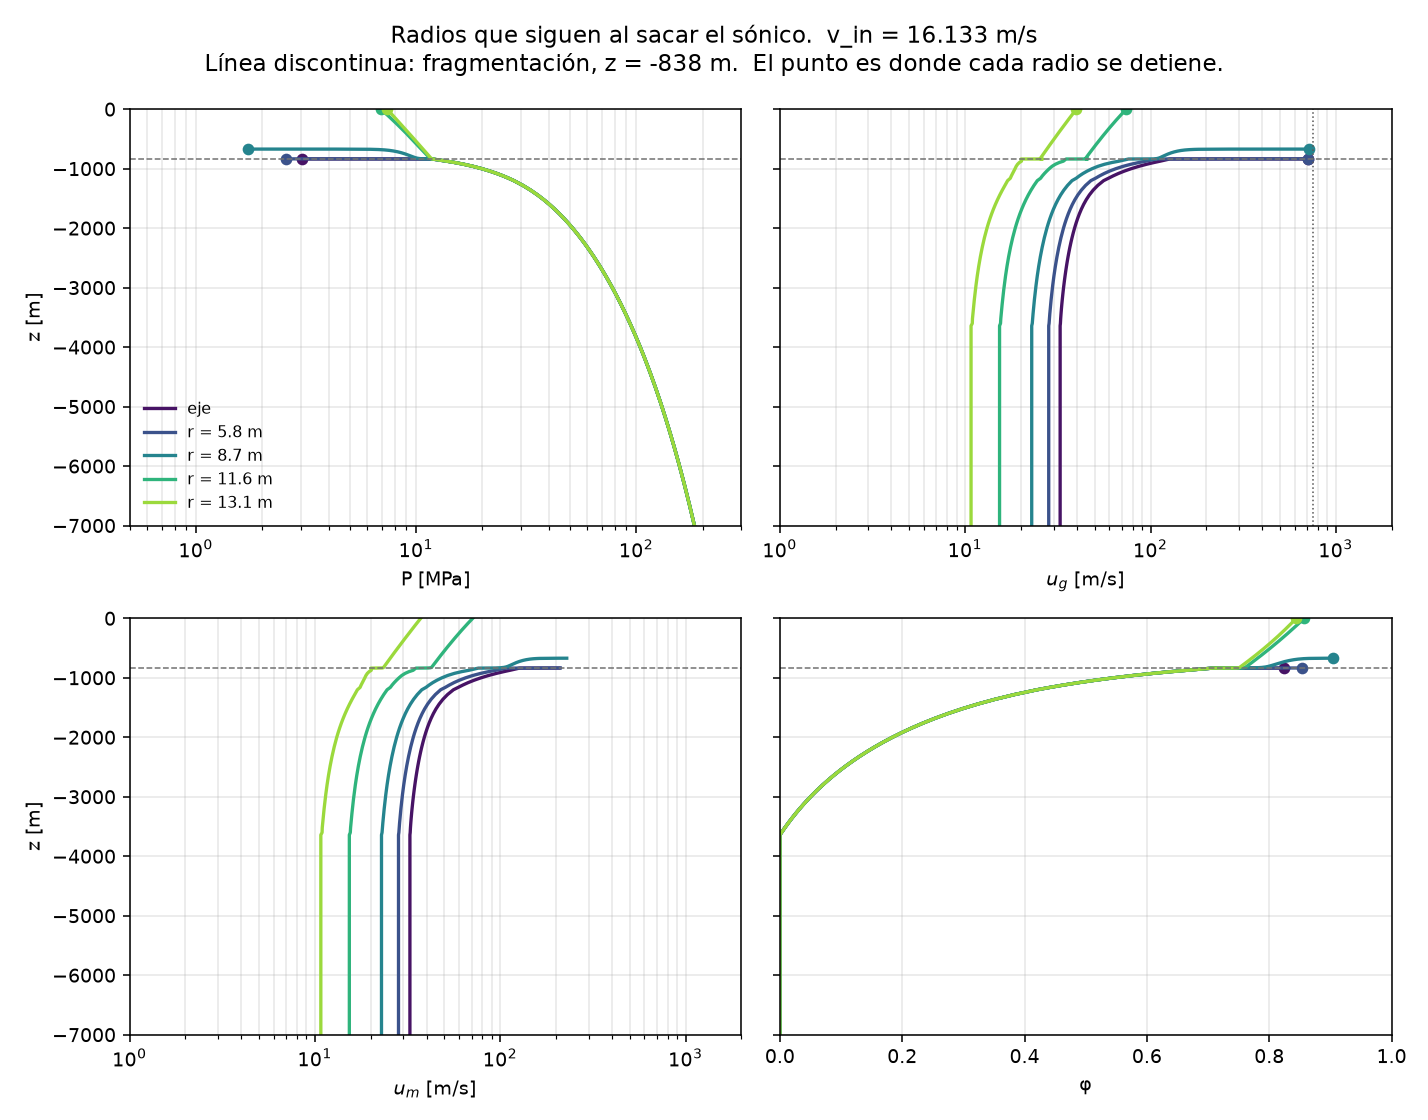
\includegraphics[width=\textwidth]{radios-siguen-fd.png}
\caption{Siete radios con el esquema implícito. Arriba, velocidad del
gas: las curvas interiores se cortan al acercarse a $c_s$ y las dos
exteriores siguen hasta $z=0$. Abajo, la presión de cada radio en su
último nivel.}
\label{fig:radios}
\end{figure}

\section{Momento radial, todavía sin correr}

Si $P=P(r,z)$, entonces $\p_r P\neq 0$ y aparece velocidad radial. Para
conservar la masa de cada fase hacen falta $u_{r,m}$ y $u_{r,g}$, y la
continuidad deja de ser $q(r)$ constante:
\[
\frac{\p}{\p z}(\rho\,\phi\,u_z)
  +\frac{1}{r}\frac{\p}{\p r}(r\,\rho\,\phi\,u_r)=0.
\]
Entran dos ecuaciones de masa y dos de momento radial, además de las
axiales. El $q(r)$ congelado de Thomas deja de describir el tramo en
cuanto hay flujo de una corona a otra.

\end{document}
